\section{Lecture 1}
\begin{itemize}
    \item A \textbf{vector} is a quantity with a magnitude, a direction, and units.
    \item A \textbf{scalar} is a quantity with a magnitude, a sign, and units.
    \begin{idea}
        At the heart of linear algebra is two operations and they both deal with vectors. We \emph{add} vectors and we multiply vectors by scalars.
    \end{idea}
    \item We can draw a vector from point $P$ to point $Q$ by drawing an arrow:
    \begin{center}
        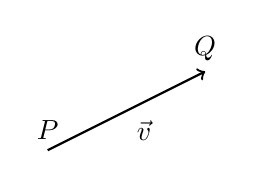
\begin{tikzpicture}[x=1cm, y=1cm]
            % Axes
            % \draw [<->] (-3,0) -- (3,0) node [at end, right] {$x$};
            % \draw [<->] (0,-3) -- (0,3) node [at end, left] {$y$};
        
            % Vectors
            \draw [->, thick] (0,0) node[above] {$P$} -- (2,1) node[above] {$Q$} node[midway,below right] {$\vec{v}$};
        \end{tikzpicture}
    \end{center}
    where $P$ is the \textbf{tail} and $Q$ is the \textbf{head} of the vector. The vector can be written algebraically as:
    \begin{equation}
        \vec{v}=\vec{PQ}
    \end{equation}
    Note that this is not equal to:
    \begin{equation}
        \vec{PQ} \neq \overrightarrow{QP}
        \label{eq:}
    \end{equation}
    because even though their magnitudes are the same, their direction is not.
    \item We can draw a two-dimensional vector in $\mathbb{R}^2$ by translating the vector $\vec{v}$ to the origin (since we are not changing direction or magnitude).
    \begin{center}
        \begin{tikzpicture}[x=1cm, y=1cm]
            Axes
            \draw [<->] (0,0) -- (3,0) node [at end, right] {$x$};
            \draw [<->] (0,0) -- (0,3) node [at end, left] {$y$};
            % node[below] {$O$}

            % Vectors
            \draw [->, thick] (0,0) node[below] {$P$} -- (2,1) node[above] {$Q$} node[midway,above] {$\vec{v}$};

            \draw[dashed] (2,0) node[below] {$v_1$} -- (2,1);
            \draw[dashed] (0,1) node[left] {$v_2$} -- (2,1);
        \end{tikzpicture}
    \end{center}
    By breaking it up into components, we can write $\vec{v}$ as a column vector:
    \begin{equation}
        \vec{v} = \begin{bmatrix}
            v_1 \\ v_2
        \end{bmatrix}
        \label{eq:}
    \end{equation}
    Note that this is not the same as a row vector:
    \begin{equation}
        \begin{bmatrix}
            v_1 \\ v_2
        \end{bmatrix}
        \neq 
        \begin{bmatrix}
            v_1 & v_2
        \end{bmatrix}
        \label{eq:}
    \end{equation}
    \item To add two vectors, we can add them components wise:
    \begin{equation}
        \vec{v}+\vec{w}=\begin{bmatrix}
            v_1 \\ v_2
        \end{bmatrix}+\begin{bmatrix}
            w_1 \\ w_2
        \end{bmatrix}=\begin{bmatrix}
            v_1+w_1 \\ v_2+w_2
        \end{bmatrix}
        \label{eq:}
    \end{equation}
    and similarly for subtraction:
    \begin{equation}
        \vec{v}-\vec{w}=\begin{bmatrix}
            v_1 \\ v_2
        \end{bmatrix}-\begin{bmatrix}
            w_1 \\ w_2
        \end{bmatrix}=\begin{bmatrix}
            v_1-w_1 \\ v_2-w_2
        \end{bmatrix}
        \label{eq:}
    \end{equation}
    \item To multiply a vector by a scalar, we multiply each component by that scalar:
    \begin{equation}
        c\vec{v} = \begin{bmatrix}
            cv_1 \\ cv_2
        \end{bmatrix}
        \label{eq:}
    \end{equation}
    \item Note that subtraction is just a combination of addition and scalar multiplication:
    \begin{equation}
        \vec{v}-\vec{w}=\vec{v}+(-1)\cdot\vec{w}
        \label{eq:}
    \end{equation}
    \item Geometrically, we can add two vectors $\vec{v}$ and $\vec{w}$:
    \begin{center}
        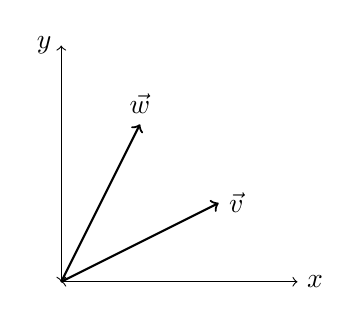
\begin{tikzpicture}[x=1cm, y=1cm]
            Axes
            \draw [<->] (0,0) -- (3,0) node [at end, right] {$x$};
            \draw [<->] (0,0) -- (0,3) node [at end, left] {$y$};
            % node[below] {$O$}

            % Vectors
            \draw [->, thick] (0,0) -- (2,1) node[right] {$\vec{v}$};
            \draw [->, thick] (0,0) -- (1,2) node[above] {$\vec{w}$};
        \end{tikzpicture}
    \end{center}
    We can do this by translating one of the vectors and add them tip to tail:
    \begin{center}
        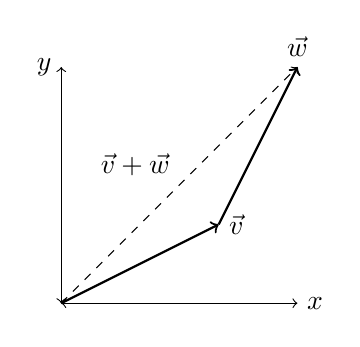
\begin{tikzpicture}[x=1cm, y=1cm]
            Axes
            \draw [<->] (0,0) -- (3,0) node [at end, right] {$x$};
            \draw [<->] (0,0) -- (0,3) node [at end, left] {$y$};
            % node[below] {$O$}

            % Vectors
            \draw [->, thick] (0,0) -- (2,1) node[right] {$\vec{v}$};
            \draw [->, thick] (2,1) -- (3,3) node[above] {$\vec{w}$};
            \draw [->, dashed] (0,0) -- (3,3) node[midway,above left] {$\vec{v}+\vec{w}$};
        \end{tikzpicture}
    \end{center}
    \item To subtract two vectors, we first flip the second vector and then add. Suppose we wish to represent $\vec{v}-\vec{w}$ geometrically, then:
    \begin{center}
        \begin{tikzpicture}[x=1cm, y=1cm]
            Axes
            \draw [<->] (0,0) -- (3,0) node [at end, right] {$x$};
            \draw [<->] (0,0) -- (0,3) node [at end, left] {$y$};
            % node[below] {$O$}

            % Vectors
            \draw [->, thick] (0,0) -- (2,1) node[above] {$\vec{v}$};
            \draw [->] (0,0) -- (1,2) node[above] {$\vec{w}$};
            \draw [->] (0,0) -- (-1,-2) node[below] {$-\vec{w}$};
            \draw [->, thick] (2,1) -- (1,-1) node[right] {$-\vec{w}$};
            \draw [->, dashed] (0,0) -- (1,-1) node[midway] {$\vec{v}-\vec{w}$};
        \end{tikzpicture}
    \end{center}
    Note that this is equivalent from adding tail to tail.
    \item To multiply a vector by a scalar, we do not change the direction but instead we change the magnitude or length. Geometrically:
    \begin{center}
        \begin{tikzpicture}[x=1cm, y=1cm]
            Axes
            \draw [<->] (-3,0) -- (3,0) node [at end, right] {$x$};
            \draw [<->] (0,-3) -- (0,3) node [at end, left] {$y$};
            % node[below] {$O$}

            % Vectors
            \draw [->, thick,color=red] (0,0) -- (3,1.5) node[above] {$1.5\vec{v}$};
            \draw [->, thick] (0,0) -- (2,1) node[above] {$\vec{v}$};
            \draw [->, thick,color=blue] (0,0) -- (1,0.5) node[above] {$0.5\vec{v}$};
            \draw [->, thick,color=green] (0,0) -- (-2,-1) node[above] {$-1\vec{v}$};
        \end{tikzpicture}
    \end{center}
    where all vectors originate from the origin.
    \item The \textbf{zero vector} is defined as:
    \begin{equation}
        \vec{0} \equiv \vec{v}-\vec{v} = \begin{bmatrix}
            0 \\ 0
        \end{bmatrix}   
        \label{eq:}
    \end{equation}
    \begin{idea}
        Scalar addition can be represented as the addition of one dimensional vectors in $\mathbb{R}^1$. For example, the number line is essentially just a coordinate axis and we can represent numbers in a similar way:
        \begin{equation}
            3=2+1
            \label{eq:}
        \end{equation}
        and geometrically:
        \begin{center}
            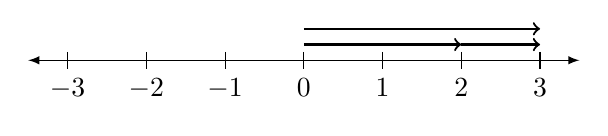
\begin{tikzpicture}
                \draw[latex-latex] (-3.5,0) -- (3.5,0) ; %edit here for the axis
                \foreach \x in  {-3,-2,-1,0,1,2,3} % edit here for the vertical lines
                \draw[shift={(\x,0)},color=black] (0pt,3pt) -- (0pt,-3pt);
                \foreach \x in {-3,-2,-1,0,1,2,3} % edit here for the numbers
                \draw[shift={(\x,0)},color=black] (0pt,0pt) -- (0pt,-3pt) node[below] 
                {$\x$};
                \draw[->,thick] (0,0.2) -- (2,0.2);
                \draw[->,thick] (2,0.2) -- (3,0.2);
                \draw[->,thick] (0,0.4) -- (3,0.4);

                \end{tikzpicture}
        \end{center}
    \end{idea}
\end{itemize}